\subsection{Đề 4}
\Opensolutionfile{ans}[ans/ans-CTST_1-OTGK1_De4-LC]
\caulc
\begin{ex}%[Câu 1]%[1D1H1-1]
	Đổi góc $270^\circ$ sang đơn vị radian.
	\choice
	{\True $\dfrac{3\pi}{2} $}
	{$\dfrac{5\pi}{2} $}
	{$\dfrac{5\pi}{6} $}
	{$\dfrac{5\pi}{3} $}
	\loigiai{Ta có $ 180^\circ=\pi$(rad) $\Rightarrow 270^\circ=\dfrac{270\cdot \pi}{180}=\dfrac{3\pi}{2}$(rad).}
\end{ex}
\begin{ex}%[Câu 2]%[1D1N1-2]
	Cho góc $\alpha \in \left(\dfrac{\pi}{2};\pi\right)$. Chọn khẳng định đúng.
	\choice
	{\True $\cos \alpha <0 $}
	{$\sin \alpha <0 $}
	{$\tan \alpha >0 $}
	{$\cot \alpha >0 $} 
	\loigiai{Giả sử điểm $M$ biểu diễn góc $\alpha \in \left(\dfrac{\pi}{2};\pi\right)$.\\ Khi đó điểm $M$ thuộc cung phần tư thứ hai.\\
		Suy ra $\sin \alpha=y_M>0$; $\cos \alpha=x_M<0$; $\tan \alpha=\dfrac{y_M}{x_M}<0 $; $\cot \alpha=\dfrac{x_M}{y_M}<0$.
	}
\end{ex}
\begin{ex}%[Câu 3]%[1D1N1-2]
	Giả sử các đẳng thức đều có nghĩa. Chọn khẳng định đúng trong các khẳng định sau.
	\choice
	{$\sin^2 \alpha+\cos^2\alpha=-1$}
	{\True $\tan \alpha \cdot \cot \alpha=1$}
	{$1+\tan^2 \alpha=\dfrac{1}{\sin^2\alpha}$}
	{$1+\cot^2 \alpha=\dfrac{1}{\cos^2\alpha}$}
	\loigiai{Theo tính chất ta có
		\begin{enumerate}
			\item $\sin^2 \alpha+\cos^2\alpha=1$.
			\item $\tan \alpha \cdot \cot \alpha=1$.
			\item $1+\tan^2 \alpha=\dfrac{1}{\cos^2\alpha}$.
			\item $1+\cot^2 \alpha=\dfrac{1}{\sin^2\alpha}$.
		\end{enumerate}
	}
\end{ex}
\begin{ex}%[Câu 4]%[1D1H1-3]
	Hàm số nào sau đây là hàm số chẵn?
	\choice
	{$y=\sin x$}
	{$y=\tan x$}
	{\True $y=\cos x$}
	{$y=\cot x$}
	\loigiai{
		Theo tính chất ta có hàm số $y=\sin x$, $y=\tan x$, $y=\cot x$ là hàm số lẻ; hàm số $ y=\cos x$ là hàm số chẵn.
	}
\end{ex}
\begin{ex}%[Câu 5]%[1D1H2-1]
	Phương trình $ \tan x=\tan\left(\dfrac{-\pi}{3}\right)$ có tất cả các nghiệm là
	\choice
	{\True $x=\dfrac{-\pi}{3}+k\pi$, $(k\in\mathbb{Z})$}
	{$x=\pm \dfrac{\pi}{3}+k\pi$, $(k\in\mathbb{Z})$}
	{$x=\dfrac{-\pi}{3}+k2\pi$, $(k\in\mathbb{Z})$}
	{$x=\dfrac{\pi}{3}+k2\pi$, $(k\in\mathbb{Z})$}
	\loigiai{
		$\tan x=\tan\left(\dfrac{-\pi}{3}\right) \Leftrightarrow x=\dfrac{-\pi}{3}+k\pi$, $(k\in\mathbb{Z})$.
	}
\end{ex}
\begin{ex}%[Câu 6]%[1D1V1-3]
	Tập nghiệm $S$ của phương trình $2\sin 2x-1=0$ là
	\choice
	{\True $S=\left\{\dfrac{\pi}{12}+k\pi; \dfrac{5\pi}{12}+k\pi\mid k\in \mathbb{Z}\right\}$}
	{$S=\left\{\dfrac{\pi}{12}+k\pi; \dfrac{-\pi}{12}+k\pi\mid k\in \mathbb{Z}\right\} $}
	{$S=\left\{\dfrac{\pi}{12}+k2\pi; \dfrac{5\pi}{12}+k2\pi \mid k \in \mathbb{Z}\right\} $}
	{$S=\left\{\dfrac{\pi}{12}+k\pi; \dfrac{11\pi}{12}+k\pi, \mid k\in \mathbb{Z}\right\}$}
	\loigiai{
		Ta có $ 2\sin 2x-1=0\Leftrightarrow\sin 2x=\dfrac{1}{2} \Leftrightarrow \hoac{&2x=\dfrac{\pi}{6}+k2\pi \\ &2x=\pi -\dfrac{\pi}{6}+k2\pi} \Leftrightarrow \hoac{& x=\dfrac{\pi}{12}+k\pi \\ & x=\dfrac{5\pi}{12}+k\pi},\, (k\in \mathbb{Z}).$
	}
\end{ex}
\begin{ex}%[Câu 7]%[1D2N2-2]
	Trong các dãy số sau, dãy nào là cấp số cộng?
	\choice
	{$2$; $3$; $5$; $7$}
	{$\dfrac{1}2$;$\dfrac{1}{4}$;$\dfrac{1}{8}$;$\dfrac{1}{16}$}
	{$1$;$0$;$0$;$0$}
	{$1$;$3$;$5$;$7$}
	\loigiai{Ta có cấp số cộng là dãy số mà mỗi số hạng kể từ số hạng thứ hai bằng số đứng liên trước cộng với một số không đổi. Số không đổi gọi là công sai của cấp số cộng, kí hiệu là $d$.\\
		Mà $3=1+2$; $5=3+ $; $7=5+2$.\\
		Vậy dãy số $1$; $3$; $5$; $7$ là cấp số cộng với công sai $d=2$.
	}
\end{ex}
\begin{ex}%[Câu 8]%[1D1N2-2]
	Cho cấp số cộng $(u_n)$ có $u_1=-3$, $u_7=21$. Khi đó công sai $d$ là
	\choice
	{$3$}
	{\True $4$}
	{$24$}
	{$\dfrac{24}{7}$}
	\loigiai{Áp dụng công thức $u_n=u_1+(n-1)d$. Khi đó
		$$
		u_7=u_1+6d \Rightarrow d=\dfrac{u_7-u_1}{6}=\dfrac{21-(-3)}{6}=4.
		$$}
\end{ex}
\begin{ex}%[Câu 9]%[1D2N3-4]
	Cho cấp số nhân $(u_n)$ có $u_1=3$, công bội $q=\dfrac{1}{3}$. Tìm $u_3$.
	\choice
	{$\dfrac{1}{9}$}
	{$\dfrac{1}{27}$}
	{$\dfrac{1}{6}$}
	{\True $\dfrac{1}{3}$}
	\loigiai{Cấp số nhân $(u_n)$ có số hạng đầu $u_1$, công bội $q$ thì công thức số hạng tổng quát của cấp số nhân là $u_n=u_1\cdot q^{n-1}$.\\
		Vậy $u_3=u_1\cdot q^2=3\cdot\left(\dfrac{1}{3}\right)^2=\dfrac{1}{3}$.}
\end{ex}
\begin{ex}%[Câu 10]%[1H4N1-1]
	Trên mặt phẳng cho $4$ điểm $A$, $B$, $C$, $D$ như hình vẽ. Ba điểm nào dưới đây không xác định một mặt phẳng?
	\begin{center}
		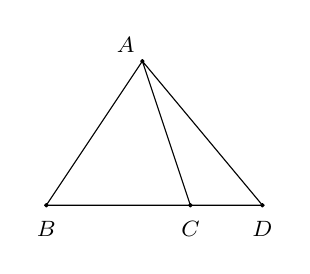
\begin{tikzpicture}[>=stealth,line join=round,line cap=round,font=\footnotesize,scale=.61]
			\path 
			(0,0) coordinate (B)
			(3,0) coordinate (C)
			(4.5,0) coordinate (D)
			(2,3) coordinate (A);
			\draw (A)--(B)--(D)--(A) (A)--(C);
			\foreach \p/\g in {B/-90, C/-90, D/-90, A/135}
			\draw[fill=black] (\p) circle (1pt) node[shift=(\g:3mm)] {$\p$};
		\end{tikzpicture}
	\end{center}
	\choice
	{$A$, $B$, $C$}
	{\True $B$, $C$, $D$}
	{$A$, $B$, $D$}
	{$A$, $C$, $D$}
	\loigiai{Vì $B$, $C$, $D$ thẳng hàng nên không xác định $1$ mặt phẳng.}
\end{ex}

\begin{ex}%[Câu 11]%[1H4N2-1]
	Chọn khẳng định đúng trong các khẳng định sau.
	\choice
	{Trong không gian, hai đường thẳng cắt nhau là hai đường thẳng không có điểm chung}
	{Trong không gian, hai đường thẳng không có điểm chung là hai đường thẳng song song}
	{Trong không gian, hai đường thẳng không có điểm chung là hai đường thẳng chéo nhau}
	{\True Trong không gian, hai đường thẳng song song là hai đường thẳng cùng nằm trong một mặt phẳng và không có điểm chung}
	\loigiai{ Trong không gian,
		\begin{enumerate}[\faCheckSquareO]
			\item Hai đường thẳng cắt nhau là hai đường thẳng có một điểm chung duy nhất.
			\item Hai đường thẳng song song là hai đường thẳng cùng nằm trong một mặt phẳng và không có điểm chung
			\item Hai đường thẳng chéo nhau là hai đường thẳng không cùng nằm trên một mặt phẳng. Suy ra hai đường thẳng chéo nhau không có điểm chung.
		\end{enumerate}
		Vậy trong không gian, hai đường thẳng không có điểm chung có thể là hai đường thẳng song song hoặc hai đường thẳng chéo nhau.
	}
\end{ex}

\begin{ex}%[Câu 12]%[1H4N3-2]
	Cho hình chóp $S.ABCD$ có đáy $ABCD$ là hình bình hành. Chọn khẳng định đúng.
	\begin{center}
		\begin{tikzpicture}[scale=1,font=\footnotesize,line join=round,line cap=round,>=stealth] 
			\path 
			(0,0) coordinate (A) 
			(-1,-1) coordinate (B) 
			($(A)+(4,0)$) coordinate (D) 
			($(B)+(4,0)$) coordinate (C) 
			($(A)+(0.5,3)$) coordinate (S)
			(intersection of A--C and B--D) coordinate (O); 
			\draw[dashed] (S)--(A)--(B) (C)--(A)--(D) (B)--(D); 
			\draw (S)--(B)--(C)--(D)--(S)--(C); 
			\foreach \p/\g in {S/135,A/135,B/-135,C/-45,D/45,O/-45} 
			\fill[black](\p) circle (1pt) ($(\p)+(\g:3mm)$) node{$\p$}; 
		\end{tikzpicture}
	\end{center}
	\choice
	{$AB \parallel (SBD)$}
	{$BC\parallel (SCD)$}
	{\True $AD \parallel (SBC)$}
	{$BD \parallel (SAC)$}
	\loigiai{Vì $ABCD$ là hình bình hành nên $AD \parallel BC$, $AD\not\subset (SBC)$ nên $AD \parallel (SBC)$.}
\end{ex}
\Closesolutionfile{ans}
\indapan{6}{ans/ans-CTST_1-OTGK1_De4-LC}
%-------------------------------------------
\Opensolutionfile{ans}[ans/ans-CTST_1-OTGK1_De4-DS]
\cauds
\begin{ex}%[1D2V1-5]
	Cho dãy số $(u_n)$ biết $u_n=\dfrac{2n+1}{n+2}, n\in\mathbb{N}^*$. Các mệnh đề sau đây đúng hay sai?
	\choiceTF
	{Hai số hạng đầu lần lượt là $u_1=1$; ${u_2}=\dfrac{5}{3}$}
	{\True Dãy số $(u_n)$ là một dãy số tăng}
	{Dãy số $(u_n)$ bị chặn trên bởi $\dfrac{33}{17}$}
	{\True Dãy số $(u_n)$ có duy nhất một số hạng nguyên}
	\loigiai{
		\begin{itemchoice}
			\itemch Ta có $u_1=\dfrac{2\cdot 1+1}{1+3}=1$; ${u_2}=\dfrac{2\cdot 2+1}{2+2}=\dfrac{5}{4}\ne\dfrac{5}{3}$.
			\itemch Ta có $u_n=2-\dfrac{3}{n+2}$ nên khi $n$ tăng thì $\dfrac{3}{n+2}$ giảm dẫn đến $u_n=2-\dfrac{3}{n+2}$ tăng.\\
			Cho nên dãy số $(u_n)$ là một dãy số tăng.
			\itemch Ta có $u_1\le u_n =2-\dfrac{3}{n+2}<2$ do $\dfrac{3}{n+2}>0$ nên $u_n=2-\dfrac{3}{n+2}<2$.\\
			Vậy dãy số $(u_n)$ bị chặn trên bởi $2$.
			\itemch Ta có $u_n=2-\dfrac{3}{n+2}$ nên $u_n$ nguyên khi $3\,\vdots\,(n+2)$ nghĩa là $\hoac{& n+2=\pm 3\\& n+2=\pm 1}\Leftrightarrow \hoac{&n=1\\&n=-5\\&n=-1\\&n=-3.}$\\
			Kết hợp với $n\in\mathbb{N}^*$ ta tìm được $n=1$.\\
			Vậy $(u_n)$ chỉ có một số hạng nguyên là $u_1=1$.
		\end{itemchoice}
	}
\end{ex}
\begin{ex}%[Câu 14]%[1D1H2-2]
	Cho góc $ \alpha \in \left(\dfrac{3\pi}{2};2\pi\right) $. Các mệnh đề sau đúng hay sai?
	\choiceTF[t]
	{\True $ \cot \alpha<0$}
	{$ \tan \left(\pi-\alpha\right)=\tan \alpha <0 $}
	{\True Nếu $ \sin \alpha =\dfrac{-3}{5}$ thì $ \cos \alpha = \dfrac{4}{5}$}
	{\True Nếu $ \sin 2\alpha=\dfrac{-\sqrt 3}{2} $ thì $ \left(\sin \alpha+\cos \alpha \right)^2 = \dfrac{2-\sqrt3}{2} $}
	\loigiai{
		\begin{itemchoice}
			\itemch Đúng. Vì giả sử điểm $ M $ biểu diễn góc $ \alpha $ thì $ M $ thuộc cung phần tư thứ tư. Suy ra $ \cos\alpha=x_M>0$, $\sin\alpha=y_M<0$, $ \tan \alpha <0 $, $\cot \alpha <0 $.
			\itemch Sai. Vì $ \tan\left(\pi-\alpha\right)=-\tan \alpha >0$.
			\itemch Đúng. Vì $ \sin^2 \alpha+\cos^2 \alpha=1 \Rightarrow \cos^2 \alpha=\dfrac{16}{25} \Rightarrow \cos \alpha =\dfrac{\pm 4}{5} $.\\
			Vì $ \alpha \in \left(\dfrac{3\pi}{2};2\pi\right) $ nên $ \cos \alpha >0 $.\\
			Vậy $ \cos \alpha =\dfrac{4}{5} $.
			\itemch Đúng. Vì $ \left(\sin \alpha+\cos \alpha\right)^2=\sin^2\alpha+2\sin\alpha\cos\alpha+\cos^2\alpha=1+\sin2\alpha=1-\dfrac{\sqrt{3}}{2}=\dfrac{2-\sqrt{3}}{2} $.
		\end{itemchoice}
	}
\end{ex}
\begin{ex}%[1D2H1-2]
	Cho dãy số $(u_n)$ biết $u_1=2$ và $u_n=\sqrt{2+u_{n-1}^2}$ với mọi $n\ge 2$.
	\choiceTF
	{Năm số hạng đầu của dãy số $(u_n)$ là $2$; $\sqrt{2}$; $2\sqrt{2}$; $2\sqrt{3}$; $2\sqrt{4}$}
	{\True Dãy số $(u_n)$ là dãy tăng}
	{\True Tích $6$ số hạng đầu của dãy số là $S=96\sqrt{35}$}
	{\True Số hạng tổng quát $u_n=\sqrt{2(n+1)}$}
	\loigiai{
		\begin{itemchoice}[t]
			\itemch Sai. Năm số hạng đầu của dãy số $(u_n)$ là $2$; $\sqrt{6}$; $2\sqrt{2}$; $\sqrt{10}$; $2\sqrt{3}$. Vậy mệnh đề ``Năm số hạng đầu của dãy số $(u_n)$ là $2$; $\sqrt{2}$; $2\sqrt{2}$; $2\sqrt{3}$; $2\sqrt{4}$'' là mệnh đề sai.
			\itemch Đúng. Dễ thấy $ u_n >0, \forall n \in \mathbb{N}^{*} $.\\ Lại có, với mọi $ n \in \mathbb{N}^{*}$ ta có $2+u_{n-1}^2>u_{n-1}^2 \Rightarrow \sqrt{2+u_{n-1}^2}>\sqrt{u_{n-1}^2}\Rightarrow u_n>u_{n-1} $.\\
			Vậy dãy số $(u_n)$ là dãy tăng.
			\itemch Đúng. Vì sáu số hạng đầu của dãy số $(u_n)$ là $2$; $\sqrt{6}$; $2\sqrt{2}$; $\sqrt{10}$; $2\sqrt{3}$; $\sqrt{14}$.\\
			Tích $6$ số hạng đầu của dãy số là $S=96\sqrt{35}$.
			\itemch Đúng. Thật vậy\\
			Ta có $u_1=\sqrt{2(1+1)}=2$ (đúng).\\
			Giả sử với $n=k$, ta có $u_k=\sqrt{2(k+1)}$.\\
			Xét $u_{k+1}=\sqrt{2(k+1+1)}=\sqrt{2(k+1)+2}=\sqrt{2+u_k^2}$ (đúng).\\
			Vậy công thức số hạng tổng quát $u_n=\sqrt{2(n+1)}$ là mệnh đề đúng.
		\end{itemchoice}
	}
\end{ex}

\begin{ex}%[Câu 16]%[2D1V2-2]
	\immini[thm]{
		Cho hình chóp $ S.ABCD$ có đáy $ABCD$ là hình bình hành tâm $O$, $M$ là trung điểm của $SC$.
		\choiceTF[t]
		{\True $OM \parallel (SAB)$}
		{$OM \parallel (SDC)$}
		{\True Mặt phẳng $(BMD)$ cắt mặt phẳng $(SAD)$ theo giao tuyến là đường thẳng đi qua $D$ và song song với $SA$}
		{Mặt phẳng $(\alpha)$ đi qua $M$ và song song với $SA$, $CD$ cắt hình chóp theo thiết diện là hình bình hành}
	}
	{
		\begin{tikzpicture}[=>stealth,line join=round,line cap=round, font=\footnotesize, scale=.7]
			\def\a{6}
			\def\goc{230}
			\def\b{4}
			\def\h{5.5}
			\path
			(0,0)coordinate (A)++(0:\a)coordinate (B)++(\goc:\b)coordinate (C)++(180:\a)coordinate(D)
			($(A)!.5!(C)$)coordinate (O)
			(O)++(100:\h)coordinate (S)		
			($(S)!.5!(C)$)coordinate (M);
			\coordinate (K) at (-1.3,4);
			\draw (S)--(B)--(C)--(D)--cycle (S)--(C);
			\draw[dashed] (O)--(S)--(A)--(C) (B)--(A)--(D)--(B) 
			;
			\foreach \x/\g in{A/160,B/0,C/-90,S/90,O/-90,D/-90,M/10}
			\fill[black](\x)circle(1pt) ($(\x)+(\g:3.5mm)$)node{$\x$}
			;
		\end{tikzpicture}
	}
	\loigiai{
		\begin{center}
			\begin{tikzpicture}[=>stealth,line join=round,line cap=round, font=\footnotesize, scale=.7]
				\def\a{6}
				\def\goc{230}
				\def\b{4}
				\def\h{5.5}
				\path
				(0,0)coordinate (A)++(0:\a)coordinate (B)++(\goc:\b)coordinate (C)++(180:\a)coordinate(D)
				($(A)!.5!(C)$)coordinate (O)
				($(A)!.5!(D)$)coordinate (N)
				($(B)!.5!(C)$)coordinate (P)
				($(S)!.5!(D)$)coordinate (Q)
				(O)++(100:\h)coordinate (S)		
				($(S)!.5!(C)$)coordinate (M);
				\coordinate (K) at (-1.3,4);
				\draw (-1.3,4)node[left]{$x$};
				\draw (S)--(B)--(C)--(D)--cycle (S)--(C) (B)--(M)--(D) (D)--(K) (Q)--(M)--(P);
				\draw[dashed] (O)--(S)--(A)--(C) (B)--(A)--(D)--(B) (M)--(O) (Q)--(N)--(P)
				;
				\foreach \x/\g in{A/160,B/0,C/-90,S/90,O/-90,D/-90,M/25,N/150,Q/100,P/0}
				\fill[black](\x)circle(1pt) ($(\x)+(\g:3.5mm)$)node{$\x$}
				;
			\end{tikzpicture}
		\end{center}
		\begin{itemchoice}
			\itemch Đúng. Vì $OM$ là đường trung bình của tam giác $SAC$ nên $OM \parallel SA$.\\
			Mà $OM\not\subset (SAB)$ nên $OM \parallel (SAB)$.
			\itemch Sai. Vì $M=OM\cap (SCD)$.
			\itemch Vì $\heva{&OM \parallel SA\\& OM \not\subset (SAD)} \Rightarrow OM \parallel (SAD)$.\\
			Mà $ OM \subset (BMD) \Rightarrow (BMD)\cap(SAD)=Dx//SA$.
			\itemch Gọi $N$, $P$ lần lượt là trung điểm của $AD$, $CB$.\\
			Suy ra $NP \parallel CD$. Mà $MO \parallel SA$.\\
			Vậy mặt phẳng $(\alpha)$ là $(MNP)$.\\
			Gọi $Q$ là trung điểm của $SD$. Suy ra $NQ \parallel SA \Rightarrow NQ \subset (\alpha)$.\\
			Suy ra $NP=(\alpha)\cap (ABCD)$; $NQ=(\alpha)\cap (SAD)$; $MQ=(\alpha)\cap(SDC)$; $PM=(\alpha)\cap(SBC)$; $NP=CD$; $ MQ=\dfrac{1}{2}CD $.\\
			Vậy thiết diện của hình chóp khi cắt bởi $(\alpha)$ là hình thang có cạnh đáy $MQ$, $NP$ và $MQ=\dfrac{1}{2}NP$.
		\end{itemchoice}
	}
\end{ex}
\Closesolutionfile{ans}
\indapan{2}{ans/ans-CTST_1-OTGK1_De4-DS}
%-------------------------------------------
\Opensolutionfile{ans}[ans/ans-CTST_1-OTGK1_De04-KQ]
\caukq
\begin{ex}%[Câu 17]%[1D2V2-7]
	Công ty cây xanh X trồng $ 496 $ cây hoa trong một khu vườn hình tam giác như sau: hàng thứ nhất trồng một cây hoa, kể từ hàng thứ hai trở đi số cây hoa trồng mỗi hàng nhiều hơn một cây so với hàng liền trước nó. Hỏi công ty cây xanh X trồng được bao nhiêu hàng cây trong khu vườn hình tam giác đó.
	\shortans{$31$}
	\loigiai{Gọi $ u_n $ là số cây hoa được trồng ở hàng thứ $ n $, với $ n \in \mathbb{N}^{*} $.\\
		Vì hàng thứ nhất trồng một cây hoa, kể từ hàng thứ hai trở đi số cây hoa trồng mỗi hàng nhiều hơn một cây so với hàng liền trước nó nên $ (u_n)$ là cấp số cộng với số hạng đầu $ u_1=1 $, công sai $ d=1 $.\\
		Tổng số cây hoa trồng được ở $ n $ hàng là 
		$$ S_n=\dfrac{\left(2u_1+(n-1)d\right)n}{2}=\dfrac{\left(2+n-1\right)n}{2}=\dfrac{\left(n+1\right)n}2.$$
		Mà công ty cần trồng $ 496 $ cây hoa nên 
		$ \dfrac{\left(n+1\right)n}2=496 \Leftrightarrow n^2+n-992=0 \Leftrightarrow n=31$ do $ (n\in  \mathbb{N}^{*}).$}
\end{ex}
\begin{ex}%[Câu 18]%[1D2V3-8]
	Anh Bảo làm việc tại công ty S năm đầu tiên với mức lương khởi điểm là $6$ triệu đồng/tháng. Từ năm thứ hai trở đi, mỗi năm lương của anh Bảo tăng thêm $15\%$ so với lương của năm trước đó. Hỏi tổng số tiền lương anh Bảo nhận được sau $5$ năm làm việc là $a$ triệu đồng. Tìm $a$ (làm tròn kết quả đến hàng đơn vị).
	\shortans{$485$}
	\loigiai{
		Tiền lương năm đầu anh Bảo nhận được là $ 6\,000\,000 \cdot 12=72\,000\,000 $ đồng.\\
		Số tiền lương của mỗi năm lập thành cấp số nhân với số hạng đầu $ u_1=72\,000\,000 $, công bội $ q=115\%=1{,}15 $.\\
		Tổng số tiền lương anh Bảo nhận được trong $ 5 $ năm làm việc là \\
		$ S_5=\dfrac{72\,000\,000 \cdot \left(1-1{,}15^5\right)}{1-1{,}15}\approx 485\,000\,000 $ (đồng) $ \approx 485 $ (triệu đồng).
	}
\end{ex}
\begin{ex}%[1D1V4-8]
	\immini{Khi đu quay hoạt động, vận tốc theo phương ngang của một cabin $M$ phụ thuộc vào góc lượng giác $\alpha = \left(Ox,OM\right)$ theo hàm số $v_x = 0{,}5\sin\alpha$ (m/s). Giá trị lớn nhất của $ v_x $ là}
	{
		\begin{tikzpicture}[scale=0.6,font=\small,line join=round,line cap=round,>=stealth]
			\tikzset{declare function={g=0;}}
			\coordinate (O) at (0,0);
			%	\coordinate[label=above right:$A$] (A) at (0:4.4);
			%	\coordinate[label=above right:$M$] (M) at (30+g:4.4);
			\pgfmathsetmacro{\gx}{60-g};
			\coordinate (v) at ($(M)+(120+g:3.3)$);
			\coordinate (vx) at ($(M)+(180:3.3*cos \gx)$);
			\draw[thick] (O) circle(4.4) (O) circle(3.53);
			\foreach \t in {0,1,...,11}{
				\draw[very thick,fill] (O)--(g+30*\t:4.4)circle(0.06);
				\begin{scope}[shift={(g+30*\t:4.4)}]
					\draw[fill=teal] (-0.27,0)--(0.27,0)--(0.36,-0.18)--(-0.36,-0.18)--cycle
					(0.32,-0.18)--(0.32,-0.54) (-0.32,-0.18)--(-0.32,-0.54)
					(-0.4,-0.54)--(0.4,-0.54)--(0.27,-1)--(-0.27,-1)--cycle;
			\end{scope}}
			\draw[fill=gray!70!yellow] (0.2,0)--(2.35,-5.53)--(3.65,-5.53)--(3.65,-6.02)--(1.95,-6.02)--(0,-0.85)--(-1.95,-6.02)--(-3.65,-6.02)--(-3.65,-5.53)--(-2.35,-5.53)--(-0.2,0)--cycle;
			\draw[fill=gray!10!yellow] (O) circle(0.34);
			\draw[fill] (-5,-5.85)--(0,-5.85) circle(0.08)--(6.4,-5.85);
			\draw[->] (-5,0)--(6.7,0) node [below]{\color{black}$x$};
			\path 
			(3.82,2.22) coordinate (M)
			($(M)-(1.8,0)$) coordinate (N)
			($(N)+(0,2.5)$) coordinate (P)
			;
			\fill[black] (M) circle(1pt) node[above right]{$M$};
			\fill[black] (N) circle(0pt) node[below left]{$\overrightarrow{v}_x$};
			\fill[black] (P) circle(0pt) node[above]{$\overrightarrow{v}$};
			\fill[black] (O) circle(2pt);
			\fill[black] (O)+(-90:0.3) circle(0pt) node[below]{$O$};
			\draw[->] (M)--(N);
			\draw[->] (M)--(P);
			\draw[dashed] (N)--(P);
			\draw (O)--(M);
			\draw[->] (O)+(0:0.8) arc (0:30:0.8) node[below right]{$\alpha$};
			\draw pic[draw, angle radius = 4mm] {right angle=O--M--P};
		\end{tikzpicture}
	}
	\shortans{$ 0{,}5 $}
	\loigiai{ Với mọi $ \alpha $ ta có\\
		$ -1\le \sin\alpha \le 1 \Rightarrow -0{,}5\le 0{,}5\sin\alpha \le 0{,}5 \Rightarrow -0{,}5 \le v_x \le 0{,}5$.\\
		Vậy giá trị lớn nhất của $v_x$ là $0{,}5$ (m/s).
	}
\end{ex}

\begin{ex}%[Câu 19]%[1D1V4-8]
	Cho vận tốc $v$ (cm/s) của một con lắc đơn theo thời gian $t$ (giây) được cho bởi công thức $v=-4\sin\left(1{,}5t+\dfrac{\pi}{3}\right)$ với $0\le t \le 2$. Xác định thời điểm vận tốc con lắc bằng $2$ cm/s. (Làm tròn kết quả đến hàng chục).
	\shortans[0]{$1{,}7$}
	\loigiai{
		Ta có
		\begin{eqnarray*}
			& & -4\sin\left(1{,}5t+\dfrac{\pi}{3}\right)=2\\
			&\Leftrightarrow & \sin\left(1{,}5t+\dfrac{\pi}{3}\right)=\dfrac{-1}{2}\\
			&\Leftrightarrow &	\hoac{&1{,}5t+\dfrac{\pi}{3}=\dfrac{-\pi}{6}+k2\pi \\ & 1{,}5t+\dfrac{\pi}{3}=\dfrac{7\pi}{6}+k2\pi}\\
			&\Leftrightarrow & \hoac{& t=\dfrac{-\pi}{3}+\dfrac{k4\pi}{3} \\ & t= \dfrac{5\pi}{9} + \dfrac{k4\pi}{3}} (k\in\mathbb{Z}).
		\end{eqnarray*}
		TH1: $ t=\dfrac{-\pi}{3}+\dfrac{k4\pi}{3}$, $0\le t \le 2 $
		$ \Rightarrow 0\le \dfrac{-\pi}{3}+\dfrac{k4\pi}{3} \le 2 \Rightarrow \dfrac{1}{4}\le k \le \dfrac{6+\pi}{4\pi} \approx 0{,}73$.\\
		Mà $ k\in \mathbb{Z} $ suy ra $ k\in \varnothing$.\\
		TH2: $ t= \dfrac{5\pi}{9} + \dfrac{k4\pi}{3}, 0\le t\le 2 $
		$ \Rightarrow 0\le \dfrac{5\pi}{9} + \dfrac{k4\pi}{3} \le 2 \Rightarrow \dfrac{-5}{3} \le t \le \dfrac{18-5\pi}{12\pi}\approx 0{,}06 $.\\
		Mà $ k\in \mathbb{Z} $ suy ra $ k=0 \Rightarrow t=\dfrac{5\pi}{9}\approx 1{,}7 $ (giây).\\
	}
\end{ex}

\begin{ex}%[Câu 21]%[1H4V1-5]
	\immini{Cho tứ diện $ABCD$ có $N$, $P$ lần lượt là trung điểm của $BC$, $BD$. Điểm $M $ là điểm thay đổi trên cạnh $AC$. Mặt phẳng $(MNP)$ cắt $AD$ tại $Q$. Giả sử $AM=kAC $. Tìm $k$ để tứ giác $MNPQ$ là hình bình hành.}
	{\begin{tikzpicture}[line cap=round,line join=round,scale=0.8]
			\coordinate[label=left:$B$] (B) at (0,0);
			\coordinate[label=right:$D$] (D) at (5.5,0);
			\coordinate[label=below:$C$] (C) at (3,-2);
			\coordinate[label=above:$A$] (A) at ($(B)+(0.5,4)$);
			\coordinate[label=below:$N$] (N) at ($(B)!0.5!(C)$);
			\coordinate[label=below:$P$] (P) at ($(B)!0.5!(D)$);
			\coordinate[label=left:$M$] (M) at ($(A)!.3!(C)$);
			%\coordinate[label=above right:$Q$] (Q) at ($(A)!.5!(D)$);
			\draw (A)--(B)--(C)--(D)--cycle (A)--(C) (N)--(M);
			\draw[dashed] (B)--(D) (N)--(P)--(M);
			\foreach \diem in {A,B,C,P,D,M,N,P}	\fill (\diem)circle(1.5pt);
	\end{tikzpicture}}
	\shortans{$0{,}5$}
	\loigiai{
		\begin{center}
			\begin{tikzpicture}[line cap=round,line join=round,scale=0.8]
				\coordinate[label=left:$B$] (B) at (0,0);
				\coordinate[label=right:$D$] (D) at (5.5,0);
				\coordinate[label=below:$C$] (C) at (3,-2);
				\coordinate[label=above:$A$] (A) at ($(B)+(0.5,4)$);
				\coordinate[label=below:$N$] (N) at ($(B)!0.5!(C)$);
				\coordinate[label=below:$P$] (P) at ($(B)!0.5!(D)$);
				\coordinate[label=left:$M$] (M) at ($(A)!.5!(C)$);
				\coordinate[label=above right:$Q$] (Q) at ($(A)!.5!(D)$);
				\draw (A)--(B)--(C)--(D)--cycle (A)--(C) (N)--(M) (M)--(Q);
				\draw[dashed] (B)--(D) (N)--(P)--(Q);
				\foreach \diem in {A,B,C,P,D,M,N,P,Q}	\fill (\diem)circle(1.5pt);
			\end{tikzpicture}
		\end{center}
		Vì $NP$ là đường trung bình của tam giác $BCD$ nên $NP \parallel CD $.\\
		Ta có $M$ là điểm chung của $(MNP)$ và $(ACD)$.\\
		Lại có $\heva{&NP \parallel CD\\& NP \subset (MNP)\\& CD \subset (ACD)}$\\
		$ \Rightarrow (MNP) \cap (ACD)=Mx \parallel CD$.\\
		Trong mặt phẳng $(ACD)$, gọi $Q=Mx\cap AD$ thì $Q=AD \cap (MNP)$.\\
		Suy ra tứ giác $MNPQ$ có $MQ \parallel  NP \parallel CD$ nên tứ giác $MNPQ$ là hình thang.\\
		Để tứ giác $MNPQ$ là hình bình hành thì $MQ=NP$ mà $NP=\dfrac{1}{2}CD$ nên $ MQ=\dfrac{1}{2}CD$.\\
		Vậy $MQ$ là đường trung bình của $\triangle ACD$, $M$ là trung điểm của $AC$ và $AM=\dfrac{1}{2}AC$.
	}
\end{ex}
\begin{ex}%[1H4V1-5]
	\immini[thm]{Cho hình chóp $S.ABCD$ có đáy $ABCD$ là hình vuông cạnh bằng $4$, $SB=SC=4$. Gọi $M$, $N$, $P$ lần lượt là trung điểm của $SA$, $AB$, $CD$. Gọi $Q$ là giao điểm của $(MNP)$ và $SD$. Tính diện tích của đa giác $MNPQ$. (Làm tròn kết quả đến hàng phần chục)}
	{\begin{tikzpicture}[=>stealth,line join=round,line cap=round, font=\footnotesize, scale=.7]
			\def\a{6}
			\def\goc{230}
			\def\b{4}
			\def\h{5.5}
			\path
			(0,0)coordinate (A)++(0:\a)coordinate (B)++(\goc:\b)coordinate (C)++(180:\a)coordinate(D)
			($(A)!.5!(C)$)coordinate (O)
			($(A)!.5!(B)$)coordinate (N)
			($(C)!.5!(D)$)coordinate (P)
			(O)++(100:\h)coordinate (S)		
			($(S)!.5!(A)$)coordinate (M)
			;
			\draw (S)--(B)--(C)--(D)--cycle (S)--(C) ;
			\draw[dashed] (S)--(A)--(C) (B)--(A)--(D)--(B) (M)--(N)--(P)--(M)
			;
			\foreach \x/\g in{A/160,B/0,C/-90,S/90,N/-90,D/-90,M/10,P/-90}
			\fill[black](\x)circle(1pt) ($(\x)+(\g:3.5mm)$)node{$\x$}
			;
		\end{tikzpicture}
	}
	\shortans{$ 5{,}2 $}
	\loigiai{
		\begin{center}
			\begin{tikzpicture}[=>stealth,line join=round,line cap=round, font=\footnotesize, scale=.7]
				\def\a{6}
				\def\goc{230}
				\def\b{4}
				\def\h{5.5}
				\path
				(0,0)coordinate (A)++(0:\a)coordinate (B)++(\goc:\b)coordinate (C)++(180:\a)coordinate(D)
				($(A)!.5!(C)$)coordinate (O)
				($(A)!.5!(B)$)coordinate (N)
				($(C)!.5!(D)$)coordinate (P)
				($(O)!.5!(P)$)coordinate (H)
				(O)++(100:\h)coordinate (S)		
				($(S)!.5!(A)$)coordinate (M)
				($(S)!.5!(D)$)coordinate (Q);
				%\coordinate (K) at (-1.3,4);
				%\draw (-1.3,4)node[left]{$x$};
				\draw (S)--(B)--(C)--(D)--cycle (S)--(C) (Q)--(P) ;
				\draw[dashed] (S)--(A)--(C) (B)--(A)--(D)--(B) (M)--(N)--(P) (M)--(Q)--(H)
				;
				\foreach \x/\g in{A/160,B/0,C/-90,S/90,N/-90,D/-90,M/10,Q/110,P/-90,H/-90}
				\fill[black](\x)circle(1pt) ($(\x)+(\g:3.5mm)$)node{$\x$}
				;
			\end{tikzpicture}
		\end{center}
		Vì $M$ là điểm chung thứ nhất của $(SAD)$ và $(MNP)$.\\
		Lại có $\heva{&NP \parallel AD \parallel BC\\& NP\subset (MNP)\\& AD\subset (SAD)}$\\
		$\Rightarrow(MNP)\cap (SAD)=Mx\parallel AD$.\\
		Trong $(SAD)$, gọi $Q=Mx\cap SD$ thì $Q=SD\cap (MNP)$.\\
		Vì $Mx \parallel AD$ nên $Q$ là trung điểm của $SD$ và $MQ=\dfrac{1}{2}AD=2$.\\
		Tứ giác $MNPQ$ có $MQ\parallel NP$, $MQ=2$, $NP=4$, $MN=\dfrac{1}{2}SB=2$, $QP=\dfrac{1}{2}SC=2$.\\ Suy ra tứ giác $MNPQ$ là hình thang cân.\\
		Kẻ $QH\perp NP$, $H\in NP$. Dễ thấy $PH=1 \Rightarrow QH=\sqrt{QP^2-PH^2}=\sqrt{3}$.\\
		Vậy diện tích hình thang cân $ MNPQ $ bằng $ \dfrac{\left(2+4\right)\cdot\sqrt{3}}{2}=3\sqrt{3}\approx 5{,}2$.
	}
\end{ex}
\Closesolutionfile{ans}
\indapan{6}{ans/ans-CTST_1-OTGK1_De04-KQ}